%% This is the standard `front matter' to be used with the illcdiss.cls
%% Latex2e document class
%%
%% Author: Maarten de Rijke
%% Current maintainer: Marco Vervoort
%%
%% Version: July, 2001
%%
%%
%% Amendment August, 2020 by Gianluca Grilletti: the nationality of the candidate should not be indicated in the titelblad, independently from the birth country
%%
%%
%%
%% MAKE SURE THAT THE FILE HAS BEEN PERSONALIZED BEFORE YOU
%% PRINT AND SHIP THE FINAL VERSION.  YOU CAN FIND ITEMS THAT NEED
%% TO BE PERSONALIZED BY SEARCHING FOR THE STRING ``%PERSONALIZE''
%%
%%
%%first of all the cover.
{\pagestyle{empty}
\newcommand{\printtitle}{%
{\Huge\bfseries Modelling Governance In\\[0.8cm] Complex Cyber-Infrastructures}}    %PERSONALIZE

\begin{titlepage}
\par\vskip 2cm
\begin{center}
\printtitle
\vfill
{\LARGE\bfseries Mostafa Mohajeri Parizi}                           %PERSONALIZE
\vskip 2cm
\end{center}
\end{titlepage}
%
% Skip a page to start on a right page again.
% If you're printing single-sided, simply delete    %PERSONALIZE
% the following line.
%
\mbox{}\newpage
\setcounter{page}{1}

%%the very first page: the `franse pagina'
\par\vskip 2cm
\begin{center}
\printtitle
\end{center}

%%the second page: the `illc pagina'
\clearpage
\par\vskip 2cm
\begin{center}
ILLC Dissertation Series DS-200X-NN                 %PERSONALIZE
\par\vspace {2cm}
\illclogo{10cm}
\par\vspace {2cm}
\noindent%
For further information about ILLC-publications, please contact\\[2ex]
Institute for Logic, Language and Computation\\
Universiteit van Amsterdam\\
Science Park 107\\
1098 XG Amsterdam\\
phone: +31-20-525 6051\\
e-mail: {\tt illc@uva.nl}\\
homepage: {\tt http://www.illc.uva.nl/}
\end{center}
\vfill

% If you're supported by NWO adapt the following 6 lines;
% otherwise simply delete them.
%
\noindent%
The investigations were supported by the Netherlands 
Organization for Scientific\linebreak Research (NWO).
\par\vspace {2cm}

% If you want to add CIP data (a summary of all the data used in
% library catalogs in a standard format), uncomment the following
% three lines and add the CIP data in between
%
%\noindent%
%{\tt CIP gegevens}                                 % PERSONALIZE
%\\[4ex]                                            %PERSONALIZE

%Copyright and accreditation stuff, plus ISBN
%
\noindent%
% Copyright: put your name here
Copyright \copyright\ 200X by John B.\ Goode\\[2ex] %PERSONALIZE
% Cover design, if your cover was designed by someone else
Cover design by Bert Jones.\\                       %PERSONALIZE
%Maybe some additional info on the production of the dissertation.
%Don't forget your printing shop
Printed and bound by your printer.\\[2ex]           %PERSONALIZE
%ISBN number: ask your printing shop to obtain one for you
ISBN: 90--XXXX--XXX--X                              %PERSONALIZE

% Dedication, table of contents and acknowledgements
% are handled in the main file


%%the third and fourth page, the `titelblad' and promotores-list, will be sent to you by the Pedel. Replace the file 'titlepage_from_pedel.pdf' by what you receive.
\clearpage
% 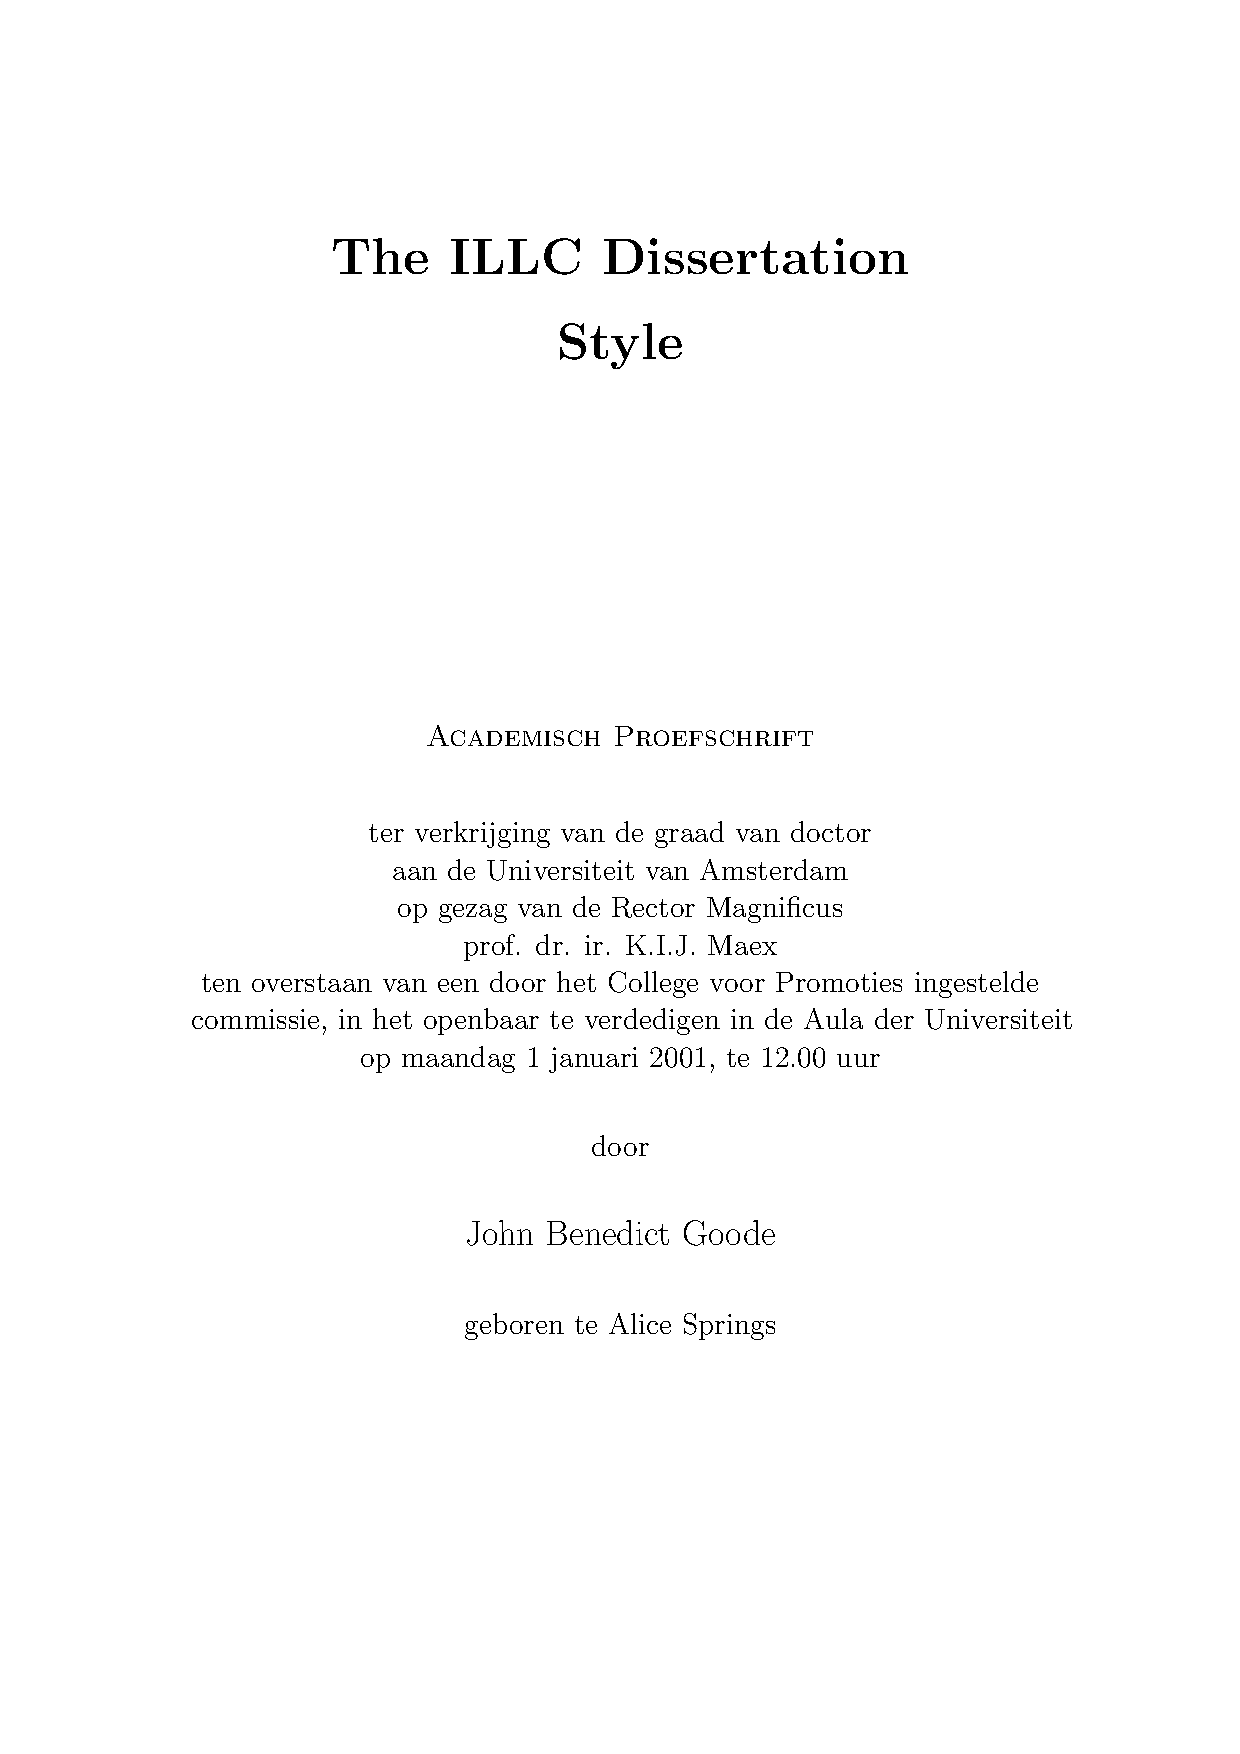
\includepdf[pages={1,2}]{titlepage_from_pedel.pdf}
%Formerly the pages were generated by the following content
 \par\vskip 2cm
 \begin{center}
 \printtitle
 \par\vspace {6cm}
 {\large \sc Academisch Proefschrift}
 \par\vspace {1cm}
 {\large ter verkrijging van de graad van doctor\\
 aan de Universiteit van Amsterdam\\
 op gezag van de Rector Magnificus\\
 prof. dr. ir. K.I.J. Maex\\                                 %PERSONALIZE
 ten overstaan van een door het College voor Promoties ingestelde\\
 \mbox{commissie, in het openbaar te verdedigen in de Aula der Universiteit}\\        %PERSONALIZE
 % Note: If your UvA PhD defense is located at the Agnietenkapel, simply write
 % 'te verdedigen in de Agnietenkapel \\', i.e. do not add 'der Universiteit'
 op maandag 1 januari 2001, te 12.00 uur \\ }        %PERSONALIZE
 \par\vspace {1cm} {\large door}
 \par \vspace {1cm} % Note: next should be your _full_ name
 {\Large Mostafa Mohajeri Parizi}                        %PERSONALIZE
 \par\vspace {1cm} % and your birthplace
 {\large geboren te Kerman} %PERSONALIZE
 % Note: NEVER include your country of birth, only the city of birth
 \end{center}
 \clearpage
 \noindent%
 {\bfseries Promotiecommissie}\\
 \\
 \begin{tabular}[t]{@{}llr}
 Promotor:      & Prof.dr.\ J.~Smith  & Universiteit van Amsterdam \\  %PERSONALIZE
 Co-promotor:   & Dr.\ T.~Jones       & Universiteit van Amsterdam \\  %PERSONALIZE
 \\
 Overige leden: & Prof. Dr. A. Aap    & Universiteit van Amsterdam \\  %PERSONALIZE
                & Prof. Dr. B. Benson & Universiteit van Amsterdam \\  %PERSONALIZE
                & Dr. C. Cornelissen  & Universiteit van Amsterdam \\  %PERSONALIZE
 \end{tabular}\\
 \\
 Faculteit der Natuurwetenschappen, Wiskunde en Informatica\\ %PERSONALIZE

\clearpage
} % Back to \pagestyle{plain}

%%%%%%%%%%%%%%%%%%%%%%%END of FRONT MATTER%%%%%%%%%%%%%%%%%%%%%%%%%%%
